\chapter{Appendix HFC}

\section{Proofs}

\subsection{Bounds between \texorpdfstring{$\rmH$}{H}, \texorpdfstring{$\rmF$}{F} and \texorpdfstring{$\rmC$}{C}}
\label{app:bounds}

\subsubsection{Bounds with backward \texorpdfstring{$\chi^2$}{chi-2} divergence}
\begin{eqnarray*}
|\rmF_{ij} - \rmH_{ij}|^2 &=& |\int \q(x, y) \big(\nabla_\theta^2 \ell(x, y)\big)_{ij} d(x, y) - \int p(x, y) \big(\nabla_\theta^2 \ell(x, y)\big)_{ij} d(x, y)|^2\\
&=& |\int \big(\q(x, y) - p(x, y)\big) \big(\nabla_\theta^2 \ell(x, y)\big)_{ij} d(x, y)|^2\\
&=& |\int \frac{\big(\q(x, y) - p(x, y)\big)}{\sqrt{p(x, y)}} \big(\sqrt{p(x, y)} \nabla_\theta^2 \ell(x, y)\big)_{ij} d(x, y)|^2\\
&\le& \int \frac{\big(\q(x, y) - p(x, y)\big)^2}{p(x, y)} d(x, y) \int p(x, y)  \big(\nabla_\theta^2 \ell(x, y)\big)_{ij}^2 d(x, y)\\
&=& \gD_{\chi^2}(\q||p) \ \E_p [ \big(\nabla_\theta^2 \ell(x, y)\big)_{ij}^2 ]
\end{eqnarray*}
Where we used Cauchy-Schwarz inequality and $\gD_{\chi^2}$ denotes the $\chi^2$ divergence.

\begin{eqnarray*}
||\rmF - \rmH||^2 &\le& \gD_{\chi^2}(\q||p) \ \E_p [ ||\rmH(x, y)||^2_2 ]
\end{eqnarray*}
Where $\rmH(x, y) \triangleq \nabla_\theta^2 \ell(x, y)$ is the empirical hessian for one sample and the $|| \cdot ||_2$ is the Frobenius norm.

In the same way
\begin{eqnarray*}
|\rmF_{ij} - \rmC_{ij}|^2 &=& |\int \q(x, y) \big(\nabla_\theta \ell(x, y) \nabla_\theta \ell(x, y)^\top \big)_{ij} d(x, y) - \int p(x, y) \big(\nabla_\theta \ell(x, y) \nabla_\theta \ell(x, y)^\top \big)_{ij} d(x, y)|^2\\
&\le& \gD_{\chi^2}(\q||p) \ \E_p [ \big(\nabla_\theta \ell(x, y) \nabla_\theta \ell(x, y)^\top \big)_{ij}^2 ]
\end{eqnarray*}

For $\rmC(x, y) \triangleq \nabla_\theta \ell(x, y) \nabla_\theta \ell(x, y)^\top$ we have

\begin{eqnarray*}
||\rmF - \rmC||^2 &\le& \gD_{\chi^2}(\q||p)\ \E_p [ ||\rmC(x, y)||^2 ]
\end{eqnarray*}

Hence
\begin{eqnarray*}
||\rmC - \rmH||^2 &\le& \gD_{\chi^2}(\q||p) \ \E_p [ ||\rmC(x, y)||^2  + ||\rmH(x, y)||^2]
\end{eqnarray*}

\subsubsection{Bounds with forward \texorpdfstring{$\chi^2$}{chi-2} divergence}
Note that in the above proof, breaking the integral in two with Cauchy-Schwarz inequality could have been done using

\begin{eqnarray*}
|\rmF_{ij} - \rmH_{ij}|^2 &=& |\int \frac{\big(\q(x, y) - p(x, y)\big)}{\sqrt{\q(x, y)}} \big(\sqrt{\q(x, y)} \nabla_\theta^2 \ell(x, y)\big)_{ij} d(x, y)|^2\\
&\le& \int \frac{\big(\q(x, y) - p(x, y)\big)^2}{\q(x, y)} d(x, y) \int \q(x, y)  \big(\nabla_\theta^2 \ell(x, y)\big)_{ij}^2 d(x, y)\\
&=& \gD_{\chi^2}(p||\q) \ \E_{\q} [ \big(\nabla_\theta^2 \ell(x, y)\big)_{ij}^2 ]
\end{eqnarray*}

Similarly
\begin{eqnarray*}
    |\rmF_{ij} - \rmC_{ij}|^2  &\le& \gD_{\chi^2}(p||\q) \ \E_{\q} [ \big(\nabla_\theta \ell(x, y) \nabla_\theta \ell(x, y)^\top \big)_{ij}^2 ]
\end{eqnarray*}
Thus 
\begin{eqnarray*}
||\rmC - \rmH||^2 &\le& \gD_{\chi^2}(p||\q) \ \E_{\q} [ ||\rmC(x, y)||^2  + ||\rmH(x, y)||^2]
\end{eqnarray*}

\subsubsection{Proof of Proposition \ref{prop:function_value}}
\label{proof:function_value}


% Let us denote by $ \tilde{ \nabla f(\theta)}$ a noisy evalution of the gradient so that $\E  \tilde{ \nabla f(\theta^{k})} =  { \nabla f(\theta^{k})}$ and $\E  \tilde{ \nabla f(\theta^{k})}  \tilde{ \nabla f(\theta^{k})}^\top = \rmC$.

From the upper bound assumption we have

\begin{eqnarray*}
f(\theta^{k+1}) &\le& f(\theta^{k}) + \nabla f(\theta^k)^\top (\theta^{k+1} - \theta^k) + \tfrac{1}{2} (\theta^{k+1} - \theta^k)^\top \rmH (\theta^{k+1} - \theta^k)\\
&=& f(\theta^{k}) - \alpha \nabla f(\theta^{k})^\top \rmM \nabla \ell(\theta^k, x) + \tfrac{\alpha^2}{2} \nabla \ell(\theta^k, x)^\top \rmM^\top \rmH \rmM \nabla \ell(\theta^k, x)\,. \\
\end{eqnarray*}

Subtracting $f(\theta^\ast)$ from both sides and taking conditional expectation we have
\begin{eqnarray*}
\E [ f(\theta^{k+1}) - f(\hat\theta^\ast)] &\le&  f(\theta^{k}) - f(\hat\theta^\ast) -\alpha \nabla f(\theta^{k})^\top \rmM\E \big[ \nabla \ell(\theta^k, x) \big] + \tfrac{\alpha^2}{2} \E \big[ \Tr \big(\rmM^\top \rmH \rmM \nabla \ell(\theta^k, x) \nabla \ell(\theta^k, x)^\top  \big) \big] \\
 &\leq&  f(\theta^{k}) - f(\hat\theta^\ast) -\alpha \nabla f(\theta^{k})^\top \rmM \nabla f(\theta^{k}) + \tfrac{\alpha^2}{2} \Tr \big(\rmM^\top \rmH \rmM (\rmC + \nabla f(\theta^k) \nabla f(\theta^k)) \big)  \\
 &=&  f(\theta^{k}) - f(\hat\theta^\ast) -\alpha \nabla f(\theta^{k})^\top (\rmM - \frac{\alpha}{2} \rmM^\top \rmH \rmM) \nabla f(\theta^{k}) + \tfrac{\alpha^2}{2} \Tr \big(\rmM^\top \rmH \rmM \rmC) \big)~,
\end{eqnarray*}
where in the second inequality we have used the covariance bound.

For $\mu_{M} \rmI \preccurlyeq \rmM - \frac{\alpha}{2} \rmM^\top \rmH \rmM$ and using the strong convexity bound $\tfrac{1}{2 \mu} \| \nabla f(\theta) \|^2 \ge f(\theta) - f(\hat\theta^\ast)$, we can simplify to 
\begin{eqnarray*}
\E [ f(\theta^{k+1}) - f(\hat\theta^\ast)] &\le&  f(\theta^{k}) - f(\hat\theta^\ast) -\alpha \mu_M \nabla f(\theta^{k})^\top \nabla f(\theta^{k}) + \tfrac{\alpha^2}{2} \Tr \big(\rmM^\top \rmH \rmM \rmC \big)  \\
&\le& f(\theta^{k}) - f(\hat\theta^\ast) -2 \alpha \mu_M \mu  \big( f(\theta^{k}) - f(\hat\theta^\ast)\big)  + \tfrac{\alpha^2}{2} \Tr \big(\rmM^\top \rmH \rmM \rmC \big)  \\
&=& \big(1 -2 \alpha \mu_M \mu\big)  \big( f(\theta^{k}) - f(\hat\theta^\ast)\big)  + \tfrac{\alpha^2}{2} \Tr \big(\rmM^\top \rmH \rmM \rmC \big)  \\
\end{eqnarray*}
Assuming $ \alpha \mu_M \mu \le \frac{1}{2}$, we have $\sum_{i=0}^k \big(1 -2 \alpha \mu_M \mu\big)^i \le \sum_{i=0}^\infty \big(1 -2 \alpha \mu_M \mu\big)^i = \frac{1}{2 \alpha \mu_M \mu} $. Therefore




\begin{eqnarray*}
\E [ f(\theta^{k+1}) - f(\hat\theta^\ast)] &\le&  f(\theta^{k}) - f(\hat\theta^\ast) -\alpha \mu_M \nabla f(\theta^{k})^\top \nabla f(\theta^{k}) + \tfrac{\alpha^2}{2} \Tr \big(\rmM^\top \rmH \rmM \rmC \big)  \\
&\le& f(\theta^{k}) - f(\hat\theta^\ast) -2 \alpha \mu_M \mu  \big( f(\theta^{k}) - f(\hat\theta^\ast)\big)  + \tfrac{\alpha^2}{2} \Tr \big(\rmM^\top \rmH \rmM \rmC \big)  \\
&=& \big(1 -2 \alpha \mu_M \mu\big)  \big( f(\theta^{k}) - f(\hat\theta^\ast)\big)  + \tfrac{\alpha^2}{2} \Tr \big(\rmM^\top \rmH \rmM \rmC \big)  \\
\end{eqnarray*}
Assuming $ \alpha \mu_M \mu \le \frac{1}{2}$, we have $\sum_{i=0}^k \big(1 -2 \alpha \mu_M \mu\big)^i \le \sum_{i=0}^\infty \big(1 -2 \alpha \mu_M \mu\big)^i = \frac{1}{2 \alpha \mu_M \mu} $. Taking full expectations and chaining inequalities we then have

\begin{eqnarray*}
\E [ f(\theta^{k}) - f(\hat\theta^\ast)] &\le& \big(1 -2 \alpha \mu_M \mu\big)^k  \big( f(\theta^{0}) - f(\hat\theta^\ast)\big)  + \tfrac{\alpha}{4 \mu_M \mu} \Tr \big(\rmM^\top \rmH \rmM \rmC \big)  \; .
\end{eqnarray*}
This concludes the proof.

\subsubsection{Convergence to limit cycles in the quadratic case}
\label{proof:quadratic}
For SGD with constant stepsize $\alpha$ and preconditioner $\rmM$, the update equation on the parameters is 
$$\theta_{t+1} = \theta_t - \alpha \rmM (\nabla f(\theta_t) + \epsilon_t) $$
In our quadratic case, $\nabla f(\theta_t) = \rmH (\theta_t - \theta^\ast)$ with $\E [\epsilon_t] = 0$ and $\E [\epsilon_t \epsilon_t^\top] = \rmS$. By defining $\delta_t = \E [\theta_t - \theta^\ast]$, we have

\begin{eqnarray*}
    \delta_{t+1} &=& (\rmI - \alpha \rmM \rmH) \delta_t \\
     &=&  (\rmI - \alpha \rmM \rmH)^{t+1} \delta_0
\end{eqnarray*}
This concludes the first result of proposition on the quadratic case.

By defining, $\rmSS_t = \E [ (\theta_t - \theta^\ast)  (\theta_t - \theta^\ast)^\top ]$, we get
% \begin{eqnarray}
% \rmSS_{t+1} &=& \rmSS_t - \E \big[ \alpha \rmM \big(\rmH (\theta_t - \theta^\ast) + \epsilon_t\big)  (\theta_t - \theta^\ast)^\top\big] \\ 
% &-& \alpha \E \big[  (\theta_t - \theta^\ast) \big(\theta_t - \theta^\ast +\epsilon_t\big)^\top \rmH \rmM^\top\big]  \\
% &+& \alpha^2\E \big[  \rmM \rmH (\theta_t - \theta^\ast) (\theta_t - \theta^\ast)^\top \rmH \rmM^\top \big] \\
% &+& \alpha^2\E \big[  \rmM \rmH \epsilon_t \epsilon_t^\top \rmH \rmM^\top \big] \\
% &=& \rmSS_t - \alpha \rmM \rmH \rmSS_t - \alpha \rmSS_t \rmH \rmM^\top + \alpha^2 \rmM \rmC \rmM^\top
% \end{eqnarray}

\begin{eqnarray}
\rmSS_{t+1} &=& \rmSS_t - \E \big[ \alpha \rmM \big(\rmH (\theta_t - \theta^\ast) + \epsilon_t\big)  (\theta_t - \theta^\ast)^\top\big] \\ 
&-& \alpha \E \big[  (\theta_t - \theta^\ast) \big(\theta_t - \theta^\ast +\epsilon_t\big)^\top \rmH \rmM^\top\big]  \\
&+& \alpha^2\E \big[  \rmM \rmH (\theta_t - \theta^\ast) (\theta_t - \theta^\ast)^\top \rmH \rmM^\top \big] \\
&+& \alpha^2\E \big[  \rmM  \epsilon_t \epsilon_t^\top  \rmM^\top \big] \\
&=& \rmSS_t - \alpha \rmM \rmH \rmSS_t - \alpha \rmSS_t \rmH \rmM^\top + \alpha^2 \rmM \rmH \rmSS_t \rmH \rmM^\top + \alpha^2 \rmM \rmS \rmM^\top\\
&=& (\rmI - \alpha \rmM \rmH) \rmSS_t (\rmI - \alpha \rmM \rmH)^\top +  \alpha^2 \rmM \rmS \rmM^\top\\
\end{eqnarray}


\subsection{Expected suboptimality for SG and Polyak momentum on quadratic functions}
\label{sec:variance_computation}
We detail here the computation of the expected suboptimality at each timestep when optimizing a quadratic function with a diagonal Hessian when the noise is also diagonal. Note that all these results apply if $\rmH$ and $\rmS$ are simultaneously diagonalizable by a change of basis.

We assume that $f$ is a quadratic with Hessian $\rmH$ and that, at each time step, we receive a gradient perturbed by a random variable $\epsilon$ with $\E[\epsilon] = 0$, $\E[\epsilon \epsilon^\top] = \rmS$.
Further, we shall assume that $\rmH$ and $\rmS$ are both diagonal. With these assumptions, the optimization occurs in each dimension independently and we can thus focus on a single dimension. We will denote by $h$ and $c$ the hessian and noise variance along that direction.

\subsubsection{Proof of proposition~\ref{prop:sg_limit}}
We can compare this result to the same setting where we use stochastic gradient with a diagonal preconditioning matrix $\rmM$. Then we get
\begin{align*}
    s_i     &= (1 - \alpha \rmM_{ii}\rmH_{ii})^2 s_i + \alpha^2 \rmM_{ii}^2 \rmS_{ii}\\
    s_i     &= \frac{\alpha \rmM_{ii} \rmS_{ii}}{2 \rmH_{ii} - \alpha \rmM_{ii}\rmH_{ii}^2}\; ,
\end{align*}
and
\begin{align*}
    \E[f(\theta_t) - f(\hat\theta^\ast)]    &= \frac{1}{2} \sum_i\frac{\alpha \rmM_{ii} \rmS_{ii}}{2 - \alpha \rmM_{ii}\rmH_{ii}} + \gO(e^{-t}) \; .
\end{align*}

Generalizing to simultaneously diagonalizable matrices, we get
\begin{align*}
    \E[f(\theta_t) - f(\hat\theta^\ast)]    &= \frac{\alpha}{2} \Tr((2\rmI - \alpha \rmM\rmH)^{-1} \rmM\rmS) + \gO(e^{-t}) \; .
\end{align*}

\subsubsection{Proof of proposition~\ref{prop:polyak_limit}}
Polyak momentum update equations are:
\begin{align}
    v_t &= \gamma v_{t-1} + \nabla f(\theta_t) + \epsilon\\
    \theta_{t+1}    &= \theta_t - \alpha v_t \; .
\end{align}
Using the quadratic assumption, we can rewrite
\begin{align*}
    v_{t+1} &= \gamma v_t + \nabla f(\theta_{t+1}) + \epsilon\\
            &= \gamma v_t + h\theta_{t+1} + \epsilon\\
            &= \gamma v_t + h\theta_t - \alpha h v_t + \epsilon \; ,
\end{align*}
and the full update can be written in matrix form
\begin{equation}
\left[
\begin{array}{c}
\theta_{t}\\
v_{t}
\end{array}
\right]
=
\left[
\begin{array}{cc}
1   &   -\alpha\\
h   &   \gamma - \alpha h
\end{array}
\right]
\left[
\begin{array}{c}
\theta_{t-1}\\
v_{t-1}
\end{array}
\right]
+
\left[
\begin{array}{c}
0\\
\epsilon
\end{array}
\right]
\end{equation}

Denoting $\displaystyle P = \left[
\begin{array}{cc}
1   &   -\alpha\\
h   &   \gamma - \alpha h
\end{array}
\right]$ and $\displaystyle S_t = [\left[
\begin{array}{c}
\theta_{t}\\
v_{t}
\end{array}
\right]\left[
\begin{array}{c}
\theta_{t}\\
v_{t}
\end{array}
\right]^T$, we have
\begin{align}
    \E[S_t | S_{t-1}]
&= PS_{t-1} P^T + \left[
\begin{array}{cc}
0   &   0\\
0   &   c
\end{array}
\right] \; .
\end{align}

If there is a limit cycle for $\displaystyle \left[
\begin{array}{c}
\theta_{t}\\
v_{t}
\end{array}
\right]$, it will satisfy
\begin{align}
    S &= PSP^T + \left[
\begin{array}{cc}
0   &   0\\
0   &   c
\end{array}
\right] \; .
\end{align}

Writing $\displaystyle S = \left[
\begin{array}{cc}
s_\theta   &   s_{v\theta}\\
s_{v\theta}   &   s_v
\end{array}
\right]$, we have
\begin{align*}
    s_\theta &= s_\theta - 2\alpha s_{v\theta} + \alpha^2 s_v\\
    s_v &=  h^2s_\theta + 2 h(\gamma - \alpha h)s_{v\theta} + (\gamma - \alpha h)^2 s_v + c\\
    s_{v\theta} &= hs_\theta + (\gamma - 2\alpha h) s_{v\theta} - \alpha(\gamma - \alpha h) s_v \; .
\end{align*}
The first equation gives $s_{v\theta} = \frac{\alpha}{2}s_v$ and the last one becomes
\begin{align*}
    \frac{\alpha}{2}s_v &= hs_\theta + (\gamma - 2\alpha h) \frac{\alpha}{2}s_v - \alpha(\gamma - \alpha h) s_v\\
    s_\theta &= \frac{\alpha (1 + \gamma)}{2h} s_v \; .
\end{align*}
Finally, the second equation gives
\begin{align*}
    s_v &=  \left(h^2\frac{\alpha (1 + \gamma)}{2h} + 2 h(\gamma - \alpha h)\frac{\alpha}{2} + (\gamma - \alpha h)^2\right) s_v + c\\
    s_v &= \frac{c}{(1 - \gamma) \left(1 + \gamma - \frac{\alpha h}{2}\right)}
\end{align*}
and
\begin{align*}
    s_\theta &= \frac{\alpha(1 + \gamma) c}{h (1 - \gamma) (2 + 2\gamma - \alpha h)} \; .
\end{align*}
Adding all dimensions together and multiplying by the Hessian to get the value function, we get
\begin{align*}
    \E[f(\theta_t) - f(\hat\theta^\ast)]    &= \frac{1}{2} \sum_i\frac{\alpha(1 + \gamma) \rmS_{ii}}{(1 - \gamma) (2 + 2\gamma - \alpha \rmH_{ii})} + \gO(e^{-t}) \; .
\end{align*}

Generalizing to simultaneously diagonalizable matrices, we get
\begin{align}
    \E[f(\theta_t) - f(\hat\theta^\ast)]    &= \frac{\alpha}{2} \frac{(1 + \gamma)}{(1 - \gamma)}\Tr\left((2 (1 + \gamma)\rmI - \alpha \rmH)^{-1} \rmS\right) + \gO(e^{-t}) \; .
\end{align}

\subsubsection{Comparison between stochastic gradient and Polyak momentum in the large noise regime}

When the desired suboptimality is small, it requires a small $\alpha$ and the two suboptimality can be approximated by
\begin{align*}
    f(\theta_t) - f(\hat\theta^\ast)    &\approx \frac{1}{4} \sum_i\frac{\alpha \rmS_{ii}}{(1 - \gamma)} + o(1) \tag{Momentum}\\
    f(\theta_t) - f(\hat\theta^\ast)    &\approx \frac{1}{4} \sum_i\alpha \rmS_{ii} + o(1)\tag{Stochastic gradient} \; ,
\end{align*}
and we see that momentum needs a stepsize $\alpha$ that is $(1 - \gamma)$ times that of stochastic gradient to achieve the same suboptimality, countering any gain. This is what we see in Table~\ref{tab:stepsize_noise}.

\section{Experimental details}

\subsection{Details on the Hessian inverse}
\label{app:inversion}
As $\rmH$ is highly degenerate in neural networks, we compute an inverse of $\rmH$ by cutting all the eigenvalues smaller than $10^{-3} \times \lambda_{max}$ where $\lambda_{max}$ is the biggest eigenvalue of $\rmH$. We observed that $10^{-3}$ and $10^{-3}$ were reasonable constants for selecting the eigenvalues of significant magnitude. Using smaller constant sometimes lead to very noisy estimates of the TIC while using a bigger constant would lead to severe underestimation of the criterion.

% \subsection{Details on the Information Matrix Equality}
% To understand the IME, one needs to show the equivalence between the two definitions of $\rmF$ eq~\ref{eq:def_f1} and eq~\ref{eq:def_f2}.

% A concise proof can be found on the Wikipedia page of the Fisher Information Matrix~\url{https://en.wikipedia.org/wiki/Fisher_information}.


\subsection{Details on the large scale experiments}
\label{app:exp_details}
These details apply for the experiments conducted in subsection~\ref{sec:neyshabur_gen}, figure~\ref{fig:large_scale_tic} and all figures in subsection~\ref{sec:exp_hfc}.

We remind the reader the setup.
\begin{itemize}
    \item 5 different architectures: logistic regression, a 1-hidden layer and 2-hidden layer fully connected network, and 2 small convolutional neural networks (CNNs, one with batch normalization~\citep{ioffe2015batch} and one without);
    \item 3 datasets: MNIST, CIFAR-10, SVHN;
    \item 3 learning rates: $10^{-2}$, $5\cdot 10^{-3}$, $10^{-3}$ using vanilla SGD with momentum $\mu = 0.9$;
    \item 2 batch sizes: $64$, $512$;
    \item 5 dataset sizes: 5k, 10k, 20k, 25k, 50k.
\end{itemize}
We train for 750k steps and compute our metrics every 75k steps.

\paragraph{Data preprocessing:} We choose to greyscale, resize to $7 \times 7$ pixels and normalize all the images in the 3 datasets used (CIFAR-10, MNIST and SVHN). This way, we can design architectures with a relatively low number of parameters.


\paragraph{Architectures:}

\begin{itemize}
    \item \texttt{mlp}: This one is a one hidden layer MLP. Input size is $7 \times 7 = 49$ and output size is $10$. The default number of hidden units is $70$. We use ReLU activations.
    \item \texttt{big\_mlp}: The architecture is the same as above but with one additional hidden layer.
    \item \texttt{logreg}: This is simple a $49 \times 10$ linear classifier.
    \item \texttt{cnn}: It is a small CNN with 3 layers. A first conv layer with kernel $3 \times 3$, $0$ padding and $15$ channels. The next layer has $20$ channels and same parameters. The last layer has $10$ channels and directly outputs the class scores.
    \item \texttt{cnn\_bn}: Same architecture as above, except for a spatial batch-norm after the second layer.
\end{itemize}

\subsection{Details on experiments of subsection~\ref{sec:neyshabur_gen}}
For these experiments we train one hidden layer MLPs on SVHN. Each points is computed by training three times with three different random seed until convergence.
In figure~\ref{fig:vary_h}, the labels are kept without corruption and we vary the hidden size layer by using $\{8, 10, 16, 20, 25, 30, 40, 50, 60, 70, 80, 100\}$ hidden units in the hidden layer.

In figure~\ref{fig:vary_corr}, we fix the number of hidden units to $70$ but we vary the labels corruption percentage from $0\%$ to $100\%$ (included) by increments of $10\%$.

The networks are trained for $150k$ gradients steps with a learning rate of $5e{-3}$ and a batch size of $256$.
We used a subset of $2000$ samples of SVHN to remain in the highly overparametrized regime, our networks were able to fit random data.


\begin{figure}[H]
  \centering
  \begin{subfigure}[b]{0.45\textwidth}
    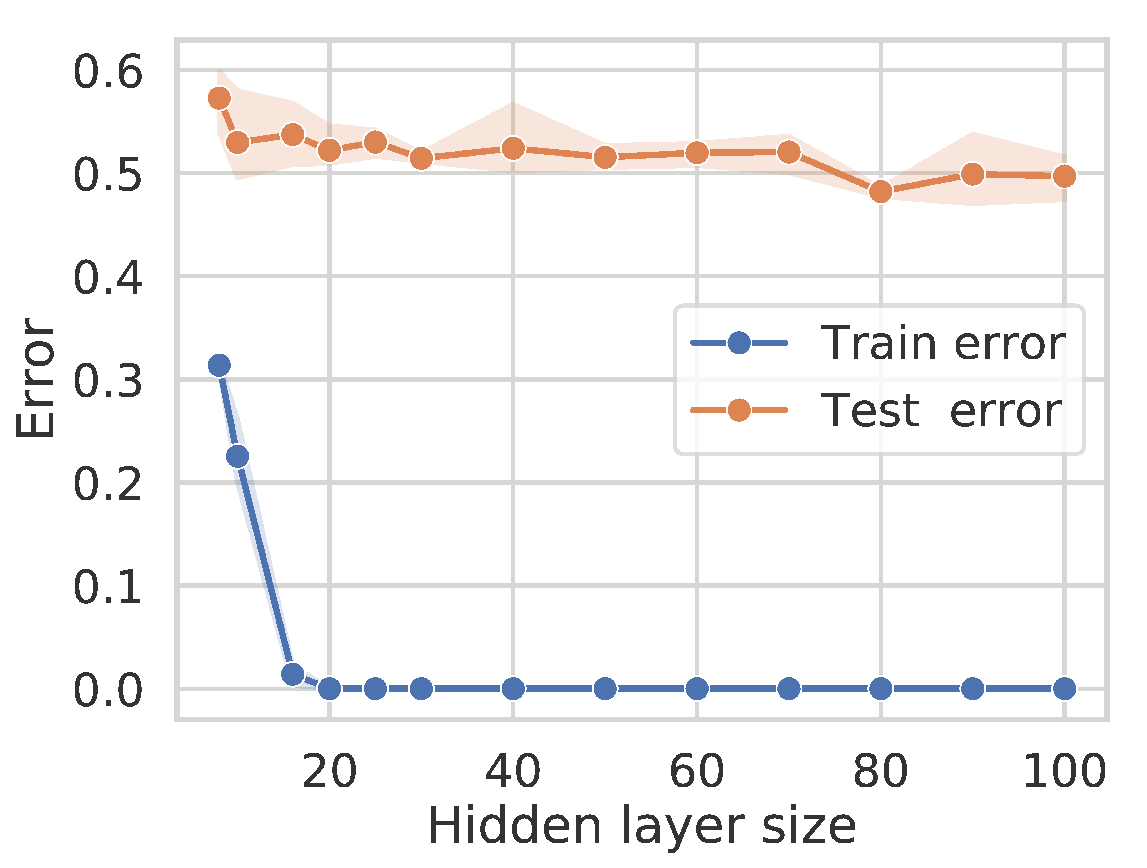
\includegraphics[width=\textwidth]{articles/hfc/traincurves_hidden_size-2.pdf}
    \caption{Varying hidden layer size.}
  \end{subfigure}
  \hfill
  \begin{subfigure}[b]{0.45\textwidth}
    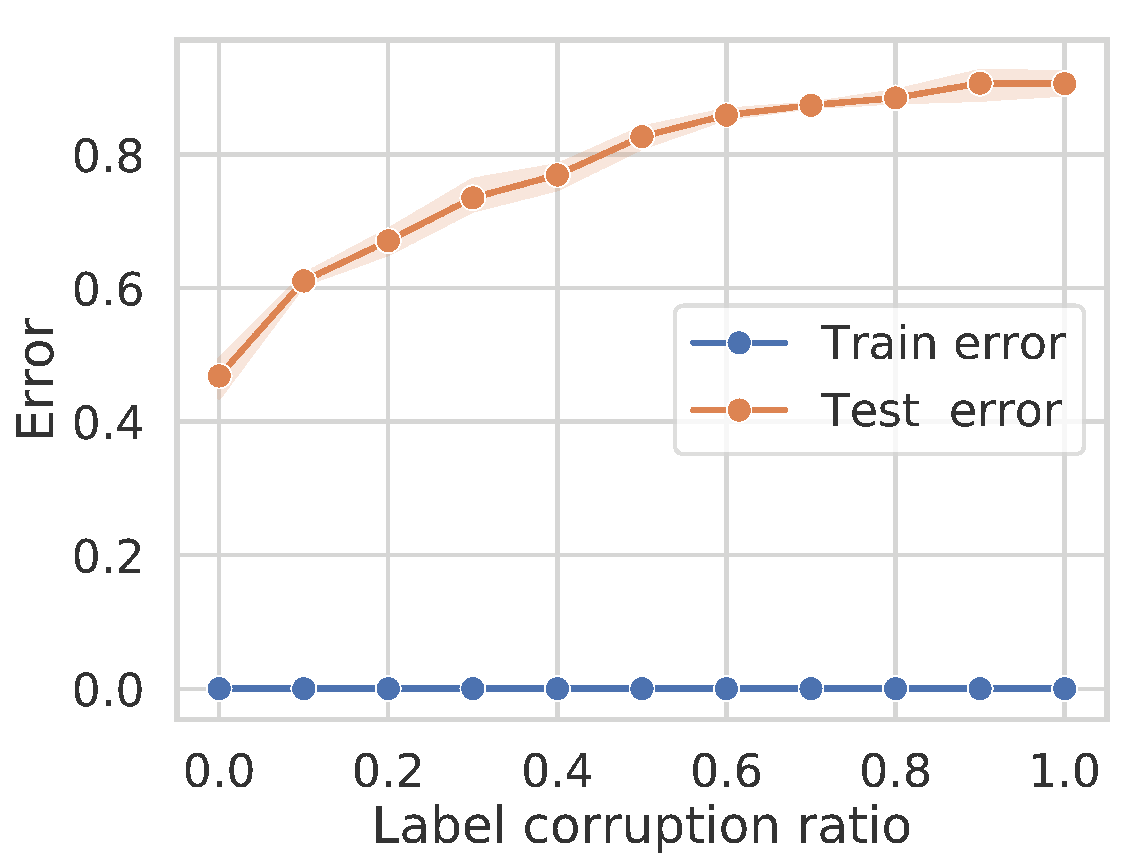
\includegraphics[width=\textwidth]{articles/hfc/traincurves_corrupt-2.pdf}
    \caption{Varying label randomization level.}
  \end{subfigure}
\caption{The train and test errors associated with the experiments~\ref{fig:vary_h} and~\ref{fig:vary_corr}. We see that while we use small networks, they are still able to fit the data completely provided we use more than 20 hidden units. This behavior mirrors the one of bigger networks.}
\end{figure}
